\documentclass{article}
\usepackage[margin=0.7in]{geometry} %LaTeX package to adjust margins
\usepackage{float} %LaTeX package to float images
\usepackage{tikz} %LaTeX package for constructing graphs
\usepackage{listings} %LaTeX package for code snippets

\begin{document}
\date{}
\title{Graphs}
\author{}
\maketitle
\graphicspath{{images/}} %configuring the graphicx package
\section*{207. Course Schedule}
\begin{flushleft}
    "There are a total of numCourses courses you have to take, labeled from 0 to numCourses - 1. You are given an array prerequisites where prerequisites[i] = [$a_i$, $b_i$] indicates that you must take course $b_i$ first if you want to take course $a_i$.
    Return \textbf{true} if you can finish all courses. Otherwise, return \textbf{false}."
\end{flushleft}
Key Concepts:
\begin{itemize}
    \item Adjacency Map
    \item DFS
    \item Cycle Detection
\end{itemize}

\begin{flushleft}
    To understand this problem it must first be noted that the schdule can be turned into a directed graph.
    We can interpret each course/prereq as a node (\textit{n}), if it is a prereq then its edge will point towards the node (course) that is leads to.
    For example, if our prerequisite list is [[1, 0], [2, 0], [3, 1]], then our graph would look like this:
\end{flushleft}
\begin{figure}[H]
    \centering
    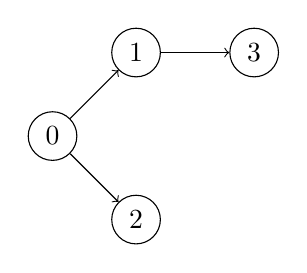
\begin{tikzpicture}[node distance={15mm}, main/.style = {draw, circle}]
        \node[main] (0) {$0$};
        \node[main] (1) [above right of=0] {$1$};
        \node[main] (2) [below right of=0] {$2$};
        \node[main] (3) [right of=1] {$3$};
        \draw[->] (0) -- (1);
        \draw[->] (0) -- (2);
        \draw[->] (1) -- (3);
    \end{tikzpicture}
    \caption{0 is the parent (\textit{prereq}) of nodes 1 and 2, and 1 is the parent of 3}
\end{figure}

\begin{flushleft}
    To construct this graph we will need to a build an \underline{adjacency map}, however, in this problem we can use a list instead.
    The index of the list will correspond to a course number which will contain a list of its prerequisites.
    Referencing the above example our adjacency list would look like:
    \begin{lstlisting}[language=Python]
    [[1, 2], [3], [], []]
    \end{lstlisting}
    Each index (prerequisite) contains a list of the courses it leads to.
\end{flushleft}
\begin{flushleft}
    The second part will be to construct out DFS algorithm which will be used to check if, given a course, it is possible to complete it (e.g. graph does not contain a cycle).
    To do this we will need the course number and a list of courses we have taken so far (visited nodes).
    We can establish the list of visited nodes outside of the function to reduce redundancy, so far our DFS function looks like:
    \begin{lstlisting}[language=python]
        visited = set()
        def containsCycle(course):
            pass #indicates incomplete function
    \end{lstlisting}
    After this we can establish our base cases where either we have no prerequisites left (succesfully completed traversal)
    or we have encountered a node already we already visited (encountered a cycle). Once we have addressed these then we can assume
    we still have more nodes to traverse and we can add the current course to our visited set.
    \begin{lstlisting}[language=python]
        visited = set()
        def containsCycle(course):
            if crs in visited:
                return True
            if adjList[crs] == []:
                return False

            visited.add(crs)
    \end{lstlisting}
    Finally, we must get the prerequisites of our course from the adjacency list and iterate over them using a for loop and then recursively running our DFS algorithm on each prereq.
    If our function encounters a cycle we can return \textbf{false} indicating that there is a cycle, otherwise the loop will terminate.
    After exiting the loop we will remove the current course from the visited list. This will allow us to empty out our visited set completely
    after running our DFS function. We can also empty out the list of prereqs for the course we called the function on to save time on future iterations
    since we know that the course can be taken. Finally we can return \textbf{false} indicating that we have not encountered any cycles.
    \begin{lstlisting}[language=python]
        def containsCycle(crs):
            if crs in visited:
                return True
            if adjList[crs] == []:
                return False

            visited.add(crs)

            for pre in adjList[crs]:
                if containsCycle(pre):
                    return True
            visited.remove(crs)
            adjList[crs] = []
            return False
    \end{lstlisting}
\end{flushleft}
\begin{flushleft}
    The rest of the problem is trivial, we just need to loop over all courses and run our DFS on each one.
    If our DFS returns \textbf{true} then we know that there is a cycle starting from that node, therefore the course cannot be taken and we can return \textbf{false}.
    Otherwise the loop will complete indicating that we can complete every course in the schedule, and we can return \textbf{true}.
\end{flushleft}
\begin{flushleft}
    The complete solution will appear as follows:
    \begin{lstlisting}[language=python]
    class Solution:
        def canFinish(self, numCourses: int, prerequisites: List[List[int]]) -> bool:
            adjList = {i:[] for i in range(numCourses)} #construct adj list
    
            for crs, pre in prerequisites:
                adjList[crs].append(pre) #map course to prereqs
    
            visited = set()
    
            def containsCycle(crs):
                if crs in visited:
                    return True #cycle detected
                if adjList[crs] == []:
                    return False  #no cycle detected
    
                visited.add(crs)
    
                for pre in adjList[crs]: #recursively check course prereqs
                    if containsCycle(pre):
                        return True
                visited.remove(crs) #dump visited set
                adjList[crs] = [] #show course can be completed (light memoization)
                return False
    
            for n in range(numCourses): #check if all courses can be completed
                if containsCycle(n):
                    return False
    
            return True    
    \end{lstlisting}
\end{flushleft}
\section*{210. Course Schedule II}
\begin{flushleft}
    "Return the ordering of courses you should take to finish all courses. If there are many valid answers, return any of them. If it is impossible to finish all courses, return an empty array."
\end{flushleft}
\begin{flushleft}
    Key Concepts:
    \begin{itemize}
        \item Topological Sort
        \item BFS or DFS
    \end{itemize}
\end{flushleft}
\begin{flushleft}
    The most important concept here is \underline{topolocial sort}, if you read the problem carefully it is clear that we need to start with the
    nodes (courses) that have no prerequisites. A topolocial sort is just ordering the nodes by degree of connections, the node(s) with 0 degrees
    of connection (e.g. parents) will come first and each child will be added after.
\end{flushleft}
\begin{flushleft}
    Like the previous problem, we will build an adjacency list, but this time do it in reverse to store which courses each prerequisite unlocks.
    We will also keep track of the incoming edges to a node in a separate array we will call \textit{indegree}. Everytime we encounter an edge from a prerequisite
    to the next node, we will increment its degree of incoming edges. The code will appear as follows:
    \begin{lstlisting}[language=python]
    def findOrder(self, numCourses: int, prerequisites: List[List[int]]):
        courses = {i:[] for i in range(numCourses)}
        indegree = [0] * numCourses #incoming edges to a node (incoming degree)

        for nxt, pre in prerequisites: #nxt indicating the next node after the prereq
            courses[pre].append(nxt)
            indegree[nxt] += 1
    \end{lstlisting}
\end{flushleft}
\begin{flushleft}
    Finally, we will construct a queue and add all nodes with no incoming edges to it (all disjoint graphs). After that we will
    perform a basic BFS similar to the DFS we did in the original course schdule problem. The only difference will be that in this one
    we will only add a course to the queue when we have satisfied all of its prerequisites (e.g. its indegree is 0). How we do this
    will be clear in the full solution code below:
    \begin{lstlisting}[language=python]
    class Solution:
        def findOrder(self, numCourses: int, prerequisites: List[List[int]]):
            courses = {i:[] for i in range(numCourses)}
            indegree = [0] * numCourses #incoming edges to a node (incoming degree)

            for nxt, pre in prerequisites: #nxt indicating the next node
                courses[pre].append(nxt)
                indegree[nxt] += 1
            
            q = collections.deque()
            for i in range(numCourses): #add all courses w/ no prereqs
                if indegree[i] == 0:
                    q.append(i)

            path = []
            while q:
                cur = q.popleft()
                path.append(cur)
                
                for nxt in courses[cur]:
                    indegree[nxt] -= 1 #we have satisfied a prereq
                    if indegree[nxt] == 0:
                        q.append(nxt)        
            
            return path if len(path) == numCourses else []
    \end{lstlisting}
\end{flushleft}
\end{document}